\chapter{adolecencia}
Muy bien lleando ala etapa de la adolecencia yo cambie muchas cosas de mi fisico me sentia mas algo y con mas masa muscular 
que en mi puberdad,yo no sabia que esta en la etapa de mi adolecencia.
si no que la mayoria de gente me decia que esta etapa es de los 14-17 años, igual decian que en esta etapa es cuando te pones melalcolico de echo me mosgraban una tabla como la siguiente
\begin{table}
	\begin{tabular}{|c|c|}
	\hline
	etapa&años\\
	niñes&5-13 años\\
	pubertad&14-17 años\\
	adultos&18-54 años\\
	tercera dedad&65años en adelante\\
	\hline
	\end{tabular}
	\caption{etapas de la vida}
	\label{etapas.com}
\end{table}
esta table me la memorice toda mi vida pero lo que decian de la melalcolia nunca me sucedio jeje
:D
ellos decian que iva a estar asi:

\begin{figure}[H]
\centering
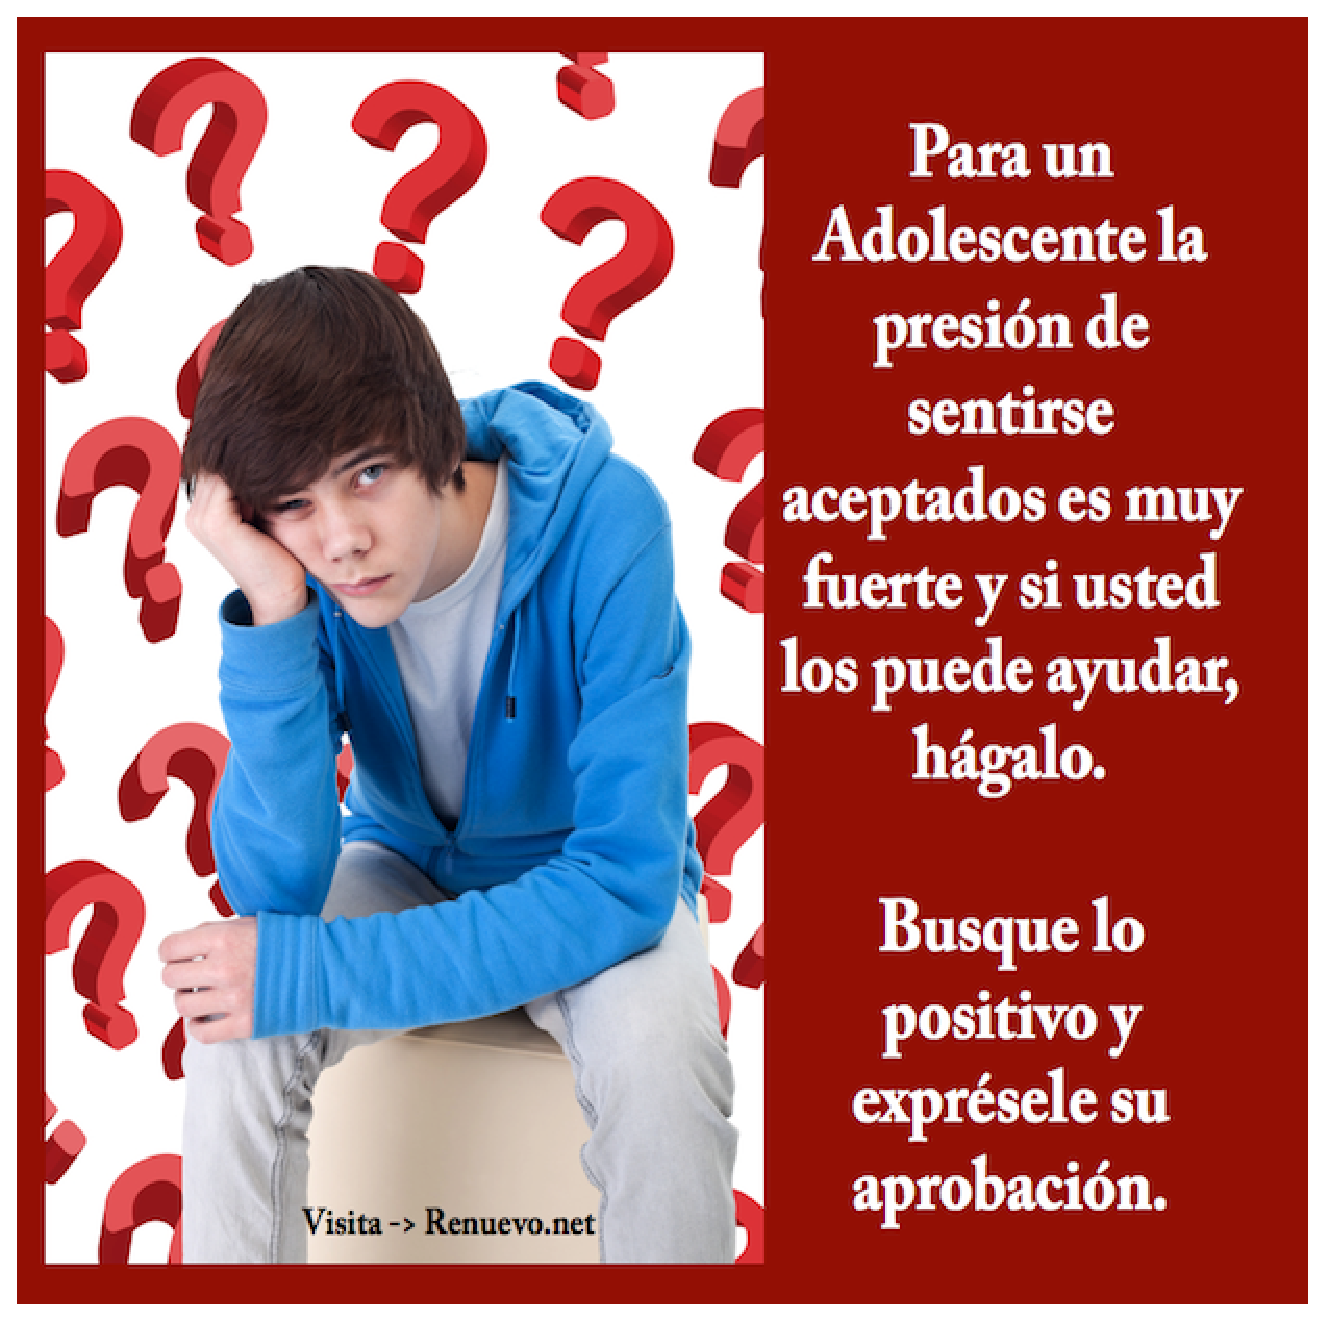
\includegraphics[width=1\textwidth]{fiveChapter/adolecente.eps}
\caption{mi adolecencia}
\label{adolecencia}
\end{figure}

pero al contrario simpre pense en viajar a estos lugares
\begin{itemize}
	\item Egipto
	\item Inglaterra
	\item Europa
	\item Mexico
		\begin{itemize}
			\item Cancun
			\item Yucatan
		\end{itemize}
	\item entre otros lugares
\end{itemize}
